\chapter{Additional Work: Extending to a Second Domain}
\label{ch:breast}

Everything reported up to this point concerns a single dataset and a single
pathology: binary pneumonia classification on RSNA chest radiographs. This
short chapter documents work that sits outside the six work packages of
Chapter~\ref{ch:context} --- a self-initiated extension, undertaken once the
core RSNA pipeline and its held-out-validation apparatus were in place, to
test whether the method and, more importantly, its \emph{evaluation
discipline} generalise beyond chest radiography at all. It should be read as
exactly that: additional, exploratory work, reported with the same honesty
as Chapter~\ref{ch:results}, not as a second fully-validated result standing
alongside the main one.

\section{Motivation}

Section~\ref{sec:heldout} established the internship's central lesson: a
counterfactual system can report near-perfect validity against the
classifier that guided it while having learned almost nothing about the
target pathology. That lesson is only as strong as its generality. A single
success --- or, here, a single negative result --- on one dataset, one
modality and one pretrained model zoo leaves open the possibility that the
finding was an artefact of RSNA, of TorchXRayVision, or of pneumonia
specifically.

Mammography was chosen as the second domain precisely because it shares as
little as possible with the first. It is a different imaging modality, it
has no representation at all in TorchXRayVision's eighteen pathology
labels, and its natural binary task --- malignant versus benign lesion ---
is semantically different from RSNA's healthy-versus-diseased framing, as
discussed in Section~\ref{sec:breast_semantics}. If the pipeline's
architecture and its habit of distrusting its own validity number survive a
change this large, that is much stronger evidence than a second run on a
second chest-radiograph corpus would have been.

\section{A Domain-Registry Architecture}

Before this extension, three things that logically belong together were
scattered across unrelated parts of the system: the dataset and its label,
the pathology head the classifier guidance targets, and which clinical
metrics are even meaningful for that pathology. Changing the dataset without
also changing the other two silently produces nonsense --- guidance toward
the wrong disease, or a cardio-thoracic ratio reported for an anatomy that
has no heart in frame.

A domain-registry abstraction was introduced to bind all three together,
with a set of optional construction hooks that a domain may override when
the TorchXRayVision-shaped defaults --- an XRV classifier head, a PSPNet
segmenter, CTR/SCP as the clinical metrics --- do not apply. Left unset, a
domain behaves exactly as the original single-dataset pipeline did, which
is what keeps the RSNA domain's behaviour byte-identical to the
pre-refactor version. Adding a new dataset is then a self-contained new
domain module plus a one-line registration, rather than an edit threaded
through ingestion, guidance and evaluation code.

\section{What Mammography Required Rebuilding}

Almost nothing about the TorchXRayVision-based guidance stack survives the
move to mammography, because that whole stack --- the pathology classifier,
the PSPNet lung/heart segmenter, and the FID feature extractor --- has no
breast equivalent. The mammography domain therefore supplies its own
version of every frozen component the RSNA pipeline was able to borrow for
free.

\subsection{A classifier trained from scratch}

A dedicated training procedure builds $f(\cdot)$ for this domain, since no
pretrained breast-malignancy head exists in the model zoo used elsewhere in
this project. Three backbones are trained --- a DenseNet-121, an
EfficientNet-B0~\cite{tan2019efficientnet}, and a ResNet-18; the first two
are registered as the guidance ensemble and the third is held back as the
independent validator, mirroring the guidance/validator split described in
Section~\ref{sec:heldout_method} for the chest domain. A gating step
applies a hard floor (minimum acceptable AUC of $0.65$) against each
backbone's saved validation AUC before any of them is allowed to guide
generation, failing explicitly rather than proceeding with a near-chance
classifier.

Two details of how that played out in practice matter for reading
Section~\ref{sec:breast_results}, and neither is visible from the design
above. First, the runs that produced the counterfactuals reported here were
made with \texttt{USE\_GUIDANCE\_ENSEMBLE = False}, so $f(\cdot)$ during
generation was the \emph{single} DenseNet-121 (validation AUC $0.796$), not
the two-model ensemble; the transfer denominator in
Table~\ref{tab:breast_transfer} is that single model accordingly. Second,
those saved validation AUCs are themselves optimistic: the trainer keeps the
best-scoring epoch and reports its score on the same fold it selected on, so
$0.796$ is a maximum over thirty epochs rather than a clean estimate. The
validators trained in Section~\ref{sec:breast_results} use nested folds to
avoid that, which is part of why their honest AUCs look lower.

The split is taken at the \emph{patient} level, not the image level. CBIS-DDSM
contains up to four images per patient (left/right breast, CC/MLO view) plus
one row per lesion; a random image-level split would place the same breast
in both train and validation and report a memorisation score as an AUC.

What that patient-level split does \emph{not} do --- and this is the flaw
Section~\ref{sec:breast_results} turns on --- is separate the three backbones
from \emph{each other}. All three take the same split, so the ``held-back''
ResNet-18 trains on precisely the images the guidance model trains on. It is
architecturally independent and statistically not independent at all.

\subsection{Two segmenters instead of one}

The chest pipeline's single PSPNet segmenter conflated two roles that
mammography must separate:

\begin{itemize}[leftmargin=*]
  \item An analytic (not learned) anatomy segmenter producing
        breast/pectoral/dense-tissue masks, used to gate the background
        lock exactly as the lung mask does for RSNA.
  \item A learned lesion segmenter, a U-Net~\cite{ronneberger2015unet}
        trained on CBIS-DDSM's shipped region-of-interest masks. It is
        deliberately excluded from the guidance loop, so that the
        clinical metrics computed from it stay independent of the edits
        they are measuring --- the same independence principle that
        motivated held-out validation in the first place.
\end{itemize}

\subsection{A new clinical metric suite}

CTR and SCP, the chest domain's clinical proxy metrics, have no meaning
here: there is no heart or costophrenic recess in a mammogram. Four
mammography-specific metrics were added instead.

\begin{itemize}[leftmargin=*]
  \item \textbf{LLR (Lesion Load Ratio)} --- lesion area over breast area,
        the structural analogue of CTR. Benign$\to$malignant edits are
        expected to raise it; malignant$\to$benign edits to lower it.
  \item \textbf{MSI (Margin Spiculation Index)} --- normalised boundary
        complexity (perimeter$^2$ / $4\pi\cdot$area) of the segmented
        lesion's largest component. Margin morphology is the single most
        load-bearing malignancy sign in mammography, and CBIS-DDSM labels it
        directly (spiculated/ill-defined versus circumscribed margins),
        which makes MSI \emph{calibratable on real images} in a way SCP
        never was. A dedicated calibration check is the gate: MSI must
        separate spiculated from circumscribed lesions on ground-truth
        images before it may be reported as evidence about counterfactuals
        at all. This calibration procedure was written and is part of the
        delivered pipeline, but was not run to completion within the time
        available for this additional work, so the MSI numbers in
        Section~\ref{sec:breast_results} should be read as provisional
        pending that gate.
  \item \textbf{BDC (Breast Density Contrast)} --- mean intensity of the
        segmented dense (fibroglandular) tissue. This one is a diagnostic
        rather than a success criterion, purpose-built to catch a specific
        failure this project had already seen once, on RSNA: an early
        policy version reported a Counterfactual Validity of $0.975$ while
        changing 73.6\% of all pixels at a mean absolute error of $0.036$
        --- a diffuse global brightness wash that moved the classifier
        without editing any anatomy. The mammography signature of the same
        failure is a large BDC shift paired with a flat LLR: the generator
        brightened or darkened the whole breast rather than altering a
        lesion. Section~\ref{sec:breast_results} reports exactly this
        pattern.
  \item \textbf{MOP (Marker/clip Preservation)} --- the mammography
        counterpart of FOP, and, unlike FOP, computable offline: surgical
        clips and skin markers are small, saturated, high-contrast metal
        objects that a simple blob detector can find without a trained
        model, sidestepping FOP's dependency on a device detector that does
        not exist for this project.
\end{itemize}

\section{Dataset and Label Semantics}
\label{sec:breast_semantics}

CBIS-DDSM (Curated Breast Imaging Subset of DDSM)~\cite{lee2017cbisddsm} is
retrieved from a public Kaggle mirror by the same provisioning step used
for RSNA. It ships 3{,}568 mass and calcification lesion
\emph{rows}, pooled across both abnormality types. Those rows are one per
\emph{lesion}, and a mammogram may carry several, so the dataset the loader
actually yields is one row per image: \textbf{2{,}857 full mammograms from
1{,}460 patients, 1{,}277 malignant against 1{,}580 benign or
benign-without-callback} (44.7\% positive) --- a considerably less skewed
split than RSNA's 22.5\% positive rate. Earlier drafts of this chapter
quoted the lesion-row figures (``$\sim$3{,}500'', ``1{,}400 / 2{,}100'') as
if they were image counts; the image-level numbers above are the ones every
result in this chapter is computed over.

One property of the dataset changes what the resulting counterfactuals mean.
CBIS-DDSM is a curated subset of \emph{lesion} cases: every image in it
contains an abnormality, and there are no normal mammograms at all. The
binary label is therefore \textbf{malignant versus benign}, not
healthy versus diseased, and the two PPO directions are
benign$\to$malignant and malignant$\to$benign. This is stated explicitly
because it is easy to misread: a reader carrying over the chest framing
might read a successful malignant$\to$benign edit as ``the model removed
the cancer,'' when what it actually claims is the narrower, weaker
statement that the generator made an already-present lesion look benign to
the classifier.

\section{Results}
\label{sec:breast_results}

The trained system was evaluated with the same protocol as
Chapter~\ref{ch:results}: groups split by classifier confidence
($n_{\text{eval}} \le 200$ per direction), deterministic mean-action policy
rollouts.

\begin{table}[h]
\centering
\caption[Breast-domain primary metrics]{Primary evaluation metrics, mammography domain. FID compares each
counterfactual set against its own real target group. The CV row and the
held-out transfer row appear together deliberately: CV is measured against
the classifier that guided generation, and is not interpretable without an
independence check beside it. Transfer is
$\Delta_{\text{validator}}/\Delta_{\text{guidance}}$; see
Table~\ref{tab:breast_transfer} for per-validator confidence intervals.}
\label{tab:breast_results}
\begin{tabular}{@{}llrr@{}}
\toprule
\textbf{Metric} & \textbf{Definition} & \textbf{benign$\to$malig.} & \textbf{malig.$\to$benign} \\
\midrule
CV   & fraction valid ($\tau = 0.8$), \emph{vs.\ the guidance model} & 1.000 & 1.000 \\
     & \textit{mean}                       & \multicolumn{2}{c}{1.000} \\
\addlinespace
\textbf{Transfer} & \textbf{independent validators, mean} & \textbf{0.066} & \textbf{0.056} \\
     & \quad resnet18-heldout (AUC 0.723)  & 0.116 & 0.032 \\
     & \quad effnet-b0-heldout (AUC 0.693) & 0.017 & 0.080 \\
     & \quad \textit{same-corpus validator (AUC 0.988)} & \textit{0.476} & \textit{0.327} \\
\addlinespace
FID  & breast-domain features, lower better & 163.6 & 193.8 \\
IP   & MS-SSIM                             & 0.891 & 0.886 \\
IP   & HF-corr                             & 0.932 & 0.946 \\
EditConcentration & top-5\% pixel mass share (uniform baseline $0.05$) & 0.367 & 0.332 \\
     & fraction of pixels changed          & 38.2\% & 40.6\% \\
MOP  & marker preservation                 & 0.930 & 0.872 \\
\bottomrule
\end{tabular}
\end{table}

\begin{table}[h]
\centering
\caption[Breast-domain clinical proxy metrics]{Mammography clinical proxy metrics: mean within-image delta and
paired $t$-test. Significance at $\alpha=0.05$ marked with $^{\ast}$.}
\label{tab:breast_clinical}
\begin{tabular}{@{}lrr@{}}
\toprule
\textbf{Metric} & \textbf{$\Delta$ benign$\to$malig.\ ($t$, $p$)} & \textbf{$\Delta$ malig.$\to$benign ($t$, $p$)} \\
\midrule
LLR & $+0.00014$ ($t=0.04$, $p=0.970$) & $-0.00107$ ($t=-0.34$, $p=0.732$) \\
MSI & $-0.082$ ($t=-1.39$, $p=0.165$)  & $-0.055$ ($t=-1.68$, $p=0.094$) \\
BDC & $+0.0014$ ($t=0.29$, $p=0.773$)  & $+0.0154$ ($t=2.46$, $p=0.015^{\ast}$) \\
\bottomrule
\end{tabular}
\end{table}

\begin{table}[h]
\centering
\caption[Breast-domain held-out transfer]{Held-out transfer ratio by validator and direction,
$n=200$ per group. Percentile bootstrap over 10{,}000 resamples, with
numerator and denominator resampled jointly so the within-image pairing is
preserved. Verdict thresholds as in Section~\ref{sec:heldout}: below $0.15$
adversarial, below $0.5$ partial. AUC is measured on the 400 real eval
originals (190 benign / 210 malignant) against radiologist pathology; $\rho$
is rank agreement with the guidance model on those same unedited images,
which separates ``disagrees about the edit'' from ``disagrees about
everything''.}
\label{tab:breast_transfer}
\resizebox{\textwidth}{!}{%
\begin{tabular}{@{}llrrrr@{}}
\toprule
\textbf{Validator} & \textbf{Independence} & \textbf{AUC} & \textbf{$\rho$} & \textbf{benign$\to$malig.} & \textbf{malig.$\to$benign} \\
\midrule
\multicolumn{6}{@{}l}{\textit{Independent and competent --- these are the result}} \\
resnet18-heldout   & patient-disjoint & 0.723 & $+0.385$ & $0.116$ $[0.097, 0.136]$ & $0.032$ $[0.017, 0.047]$ \\
effnet-b0-heldout  & patient-disjoint & 0.693 & $+0.370$ & $0.017$ $[-0.011, 0.044]$ & $0.080$ $[0.057, 0.103]$ \\
\textbf{mean}      &                  &       &          & $\mathbf{0.066}$ & $\mathbf{0.056}$ \\
\midrule
\multicolumn{6}{@{}l}{\textit{Reported for contrast --- neither is an independence check}} \\
resnet18-cbis      & same train fold  & 0.988 & $+0.826$ & $0.476$ $[0.427, 0.526]$ & $0.327$ $[0.282, 0.373]$ \\
resnet18-cmmd      & external corpus  & 0.507 & $+0.055$ & $0.091$ $[0.071, 0.111]$ & $0.052$ $[0.034, 0.069]$ \\
effnet-b0-cmmd     & external corpus  & 0.499 & $-0.000$ & $-0.006$ $[-0.019, 0.007]$ & $0.095$ $[0.084, 0.107]$ \\
\bottomrule
\end{tabular}%
}
\end{table}

Figures~\ref{fig:breast_n2p} and~\ref{fig:breast_p2n} show representative
qualitative examples for each direction.

\begin{figure}[h]
  \centering
  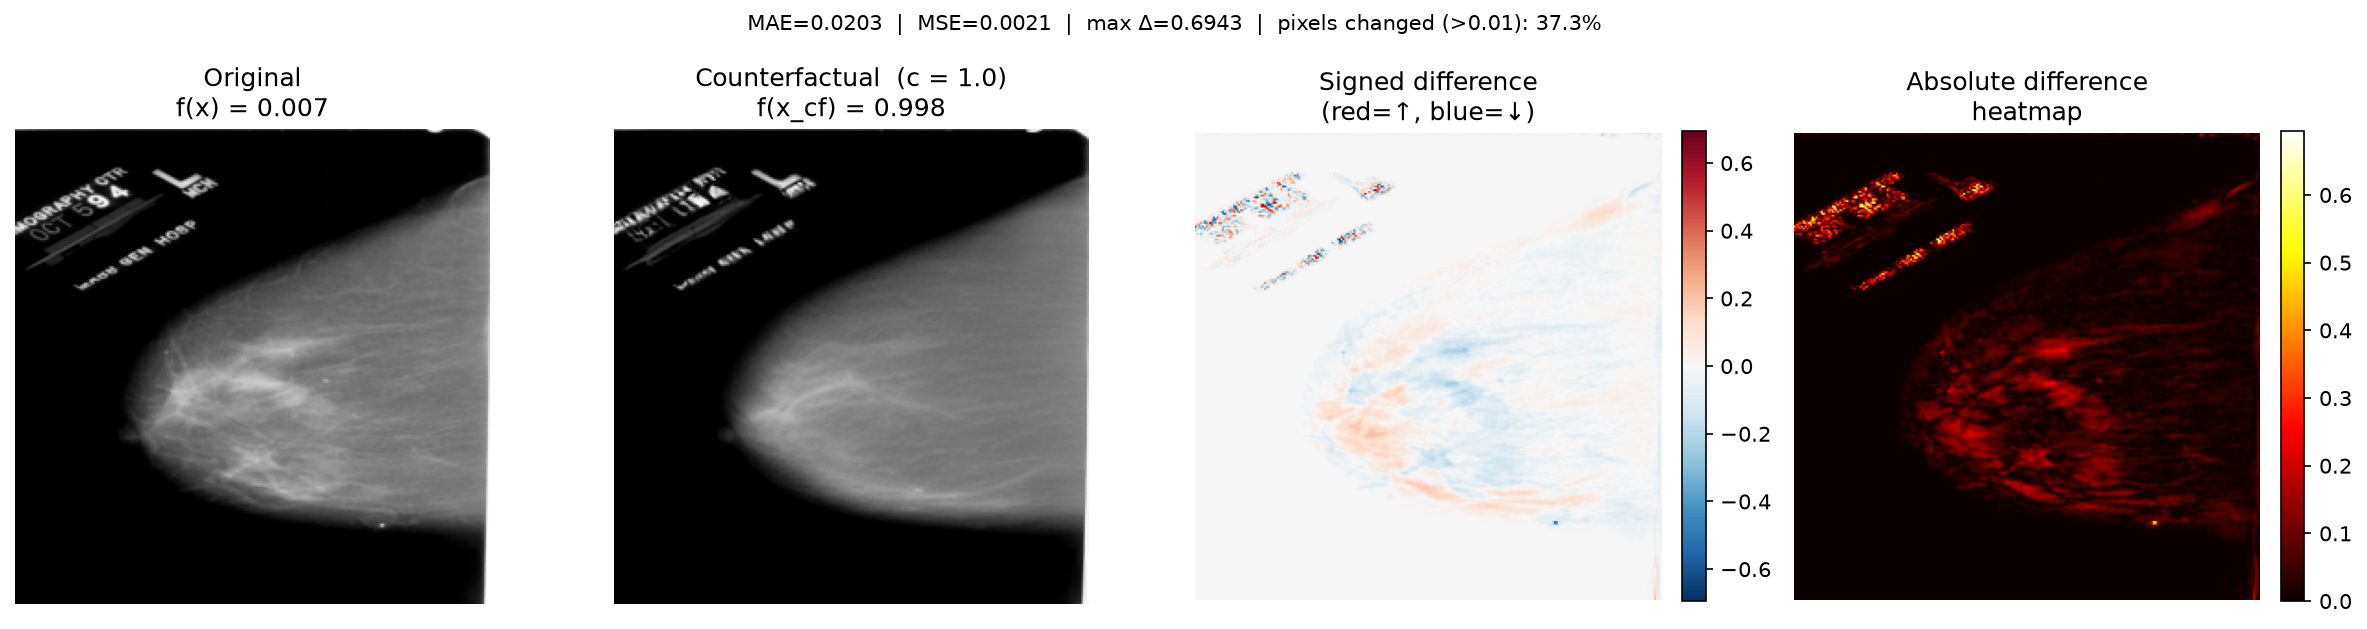
\includegraphics[width=\textwidth]{counterfactual_diff_n_to_p_breast.png}
  \caption[Breast counterfactual: benign to malignant]{\textbf{Benign $\rightarrow$ malignant.} Original, counterfactual
  targeting the malignant class, signed pixel difference, and
  absolute-difference heatmap, on the mammography domain.}
  \label{fig:breast_n2p}
\end{figure}

\begin{figure}[h]
  \centering
  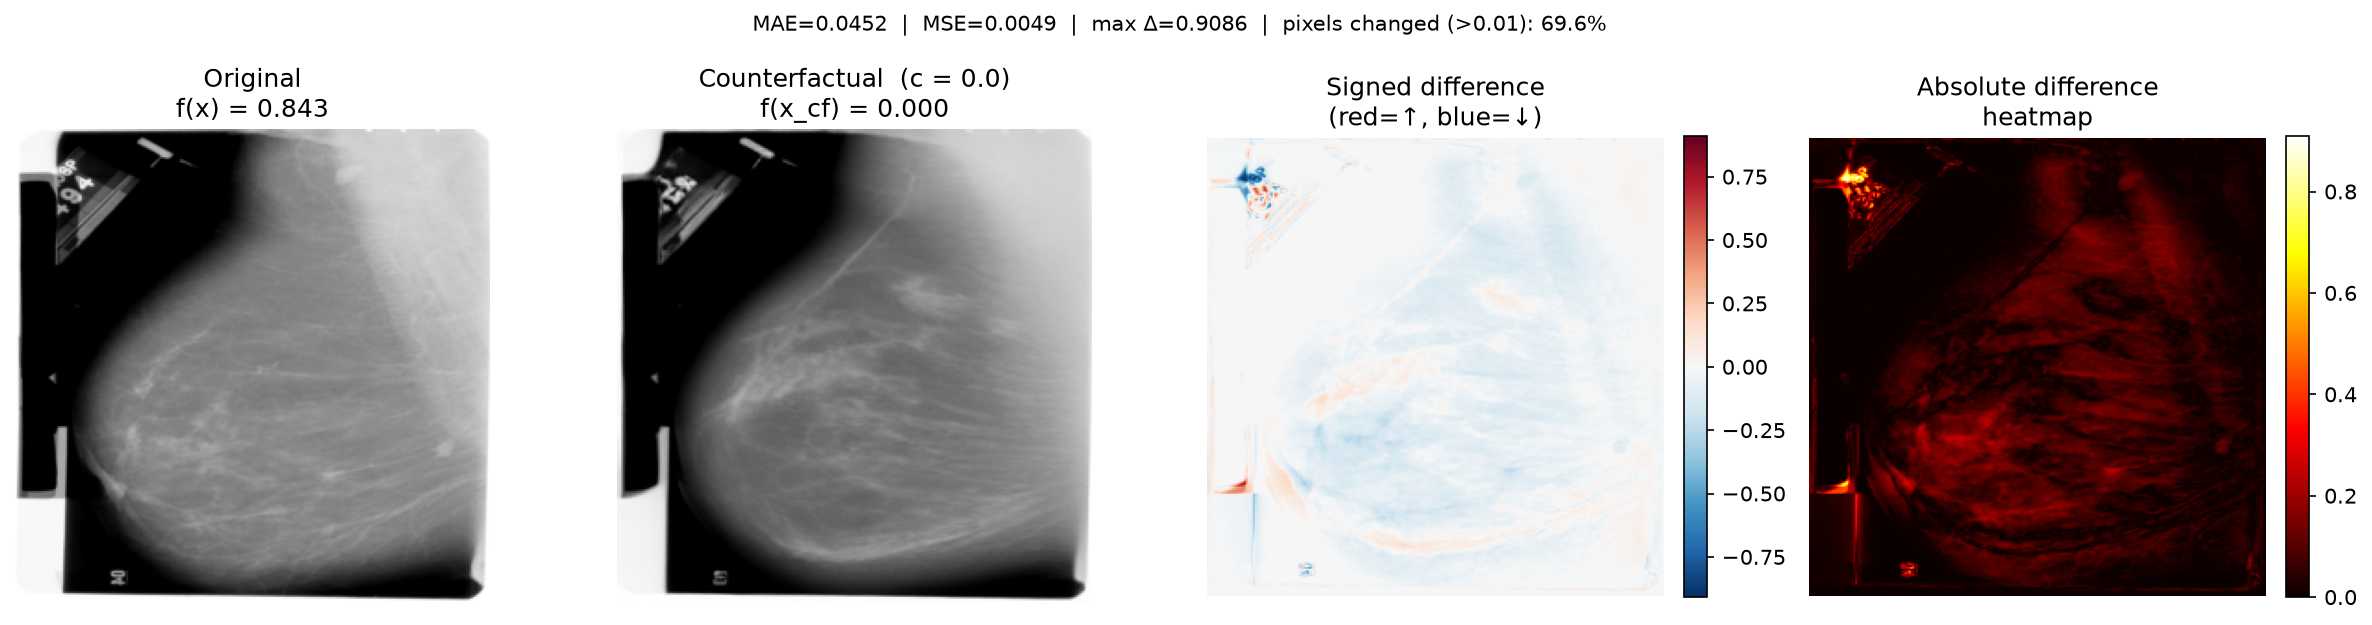
\includegraphics[width=\textwidth]{counterfactual_diff_p_to_n_breast.png}
  \caption[Breast counterfactual: malignant to benign]{\textbf{Malignant $\rightarrow$ benign.} Same four-panel layout.}
  \label{fig:breast_p2n}
\end{figure}

The guidance diagnostics recorded alongside each policy checkpoint (a
20-episode probe) show the same kind of directional specialisation
observed on RSNA: the benign$\to$malignant policy settles at a higher
guidance bias (mean $0.980$, $3.45$ refinement passes on average, average
reward $8.53$) than the malignant$\to$benign policy ($0.790$, $3.20$
passes, average reward $5.10$), indicating the two directions again
learned visibly different control strategies rather than converging to a
shared, direction-agnostic schedule.

\subsection{Reading These Numbers Honestly}

Three things in these tables should stop a reader before they are taken as a
mammography success story.

\textbf{The CV number is exactly the shape of the number that misled the
project once already, and the held-out column beside it says so.} A mean
Counterfactual Validity of $1.000$ against the guidance classifier is,
superficially, an even stronger result than RSNA's $0.975$.
Section~\ref{sec:heldout} showed that a comparably high number computed
against a guidance classifier collapsed to at most 8\% under genuinely
independent validators. The same thing happens here, and harder: against
validators that never saw the guidance model's training data and never saw
one of the 400 images they score, the counterfactuals reproduce a mean
$6.6\%$ (benign$\to$malignant) and $5.6\%$ (malignant$\to$benign) of the
guidance model's own score shift. All four bootstrap intervals in
Table~\ref{tab:breast_transfer} lie wholly below the $0.15$ adversarial
threshold, the widest reaching only $0.136$, so at $n=200$ per group this is
not a small sample failing to resolve an effect --- the adversarial regime is
positively established. In one direction the EfficientNet validator's
interval, $[-0.011, 0.044]$, contains zero, meaning no detectable malignancy
signal at all. The chest domain's \emph{worst} arm transfers at
$0.230/0.146$; mammography is more adversarial than any RSNA arm, not less.

\textbf{The validator this domain reserved was never an independence check,
and the gap shows what that was worth.} The plan in
Section~\ref{sec:heldout_method} was sound --- train three backbones, guide
with two, hold one back --- and
\texttt{DomainProfile.validate()} does enforce that the held-back model never
appears in the guidance fields. But all three were trained by
\texttt{train\_breast\_classifier.py} on \emph{one} patient-level split
(\texttt{seed}~0, \texttt{val\_frac}~0.2), so
\texttt{resnet18-breast-cbis} shares every training image with the model it
was meant to check --- and, because the eval groups were drawn from the whole
corpus, it had also been fit on 336 of the 400 eval images (84\%, spanning
304 of 362 patients). Its AUC on those images is $0.988$, against $0.723$ and
$0.693$ for validators that have not seen them: that is memorisation, not
accuracy. Reported as this domain's independence check it would have read
$0.476/0.327$ --- ``partial'' on this project's own scale, four to ten times
the honest figure. The check compared model \emph{identity}; nothing compared
training \emph{data}. That is a general lesson, not a mammography one.

\textbf{The BDC/LLR pairing reached the same conclusion first, and that
convergence is the strongest part of this result.} In the
malignant$\to$benign direction, BDC shifts significantly ($t=2.46$,
$p=0.015$) while LLR --- the metric that would move if a lesion were actually
shrinking or disappearing --- does not ($p=0.732$). That is precisely the
pattern BDC was designed to catch: a diffuse change in overall breast density
large enough to move the classifier, occurring while the segmented lesion's
relative size is statistically unchanged. Read together with an
edit-concentration figure well below what a focal, lesion-confined edit would
produce (0.33--0.37 against a uniform baseline of $0.05$, with 38--41\% of
all pixels changed), the diffuse-edit reading was already the defensible one.

The held-out transfer ratio is a second instrument with nothing
methodological in common with the first --- an independently trained
classifier rather than a statistic derived from a segmentation mask --- and
it agrees. That agreement is not a coincidence but a prediction borne out: a
diffuse density wash that moves a density-sensitive classifier without
altering the lesion is exactly the kind of edit a classifier trained on
different patients would fail to follow. Either result alone would be
suggestive; two unrelated measurements converging is what makes the reading
defensible.

\subsection{What Would Have to Be True for This to Be Wrong}

Three limits are worth stating plainly, because none of them is dissolved by
the result above.

\textbf{The independent validators are competent, not strong.} At AUC
$0.69$--$0.72$ they set a floor on how much real signal an edit must carry
before it registers, and a subtle but genuine lesion change could fall below
it. The finding is that a large adversarial component is present, not that
the disease signal is exactly zero. That ceiling is a data limit rather than
a modelling one: the only CBIS-DDSM patients no guidance backbone was fit on
number 292, and after removing every patient appearing in the eval groups the
training pool is 234 patients / 432 images, against the guidance model's
2{,}290.

\textbf{The external-corpus check was attempted and failed its own sanity
gate, and both of its AUCs are worth reporting rather than just the failing
one.} A validator trained on CMMD --- different country, different scanner
generation, no possible patient overlap --- would in principle have been the
strongest independence claim available. On its \emph{own} held-out CMMD
patients it reaches out-of-fold AUC $0.624$ (ResNet-18) and $0.635$
(EfficientNet-B0): meaningfully above chance, but already below this
project's $0.65$ floor on its native data, before CBIS-DDSM enters the
picture at all. Scored on real CBIS-DDSM images it collapses further, to
AUC $0.507$ and $0.499$ --- indistinguishable from chance --- with rank
agreement $\rho = +0.055$ and $\rho = -0.000$ against the guidance model on
the unedited originals. The scores are not degenerate (std $0.108$, a
roughly unimodal spread from $0.18$ to $0.82$), so this is not a broken
forward pass; the label mapping and the pixel-preprocessing pipeline are
byte-identical to CBIS-DDSM's. What differs is framing: CMMD's mirror ships
pre-cropped lesion patches (34.5\% near-black background) against
CBIS-DDSM's full mammograms (54.7\%), and the classifier appears to have
keyed on something in that framing rather than on transferable malignancy
signal. This was already a weak validator on its own corpus, and the drop
to chance on a different one is a domain-shift failure layered on top of a
mediocre starting point, not a strong classifier undone by nothing but
format. Either way its transfer ratios are \emph{uninterpretable} and
excluded from the mean: a classifier that cannot tell real malignant from
real benign would not follow a genuine disease edit either, so a low ratio
from it is evidence about the validator, not about the counterfactuals ---
which is why every validator here is gated on AUC before its ratio is
read at all.

\textbf{Disjointness holds at two levels of three, and the third is
arithmetically out of reach.} The ideal validator would have touched none of
the guidance model's training data, none of its validation data, and none of
the PPO rollout pool. These validators clear the first and score images they
have never seen. They do not clear the other two, and it is worth being exact
about why.

They are trained on the guidance models' \emph{validation} fold --- the 292
patients left over from the 1{,}168 the guidance model was fit on, minus the
eval-group patients, leaving 234. CBIS-DDSM contains 1{,}460 patients and the
split is 1{,}168 / 292, so excluding both folds leaves precisely zero
patients: within this corpus there is no third partition to draw from. What
that fold touched is narrow --- the guidance checkpoint was the best-scoring
epoch on it, so those images influenced \emph{which epoch was frozen}, not
what the weights learned. And the bias it introduces runs against the finding
rather than toward it: a validator sharing images with the guidance model's
selection criterion should agree with it \emph{more}, inflating transfer, not
suppressing it. The measured $0.066/0.056$ is therefore conservative.

They are also not disjoint from the PPO rollout pool, and no subset of
CBIS-DDSM could be: the environment's far-pool scan drew on the entire
2{,}857-image corpus (1{,}603 images for benign$\to$malignant plus 1{,}254
for malignant$\to$benign, which is exactly 2{,}857). Closing that last level
would mean retraining the policies on a reserved patient fold, which would
produce different counterfactuals from the ones measured here.

One caveat cuts the other way and belongs on the clinical-metric side rather
than the transfer side: BDC's $p=0.015$ does not survive Bonferroni
correction across the six clinical tests ($0.05/6 = 0.0083$). The transfer
ratio is unaffected --- it is a single pre-specified measurement, not one of
a family of six.

\section{What This Additional Work Actually Demonstrates}

This extension does not add a second validated success to the internship's
results. What it demonstrates is more useful than that, and in the end
stronger than the architecture-generalises claim it was originally written to
make.

The domain-registry architecture did carry cleanly to a modality that shares
essentially nothing with chest radiography. But the substantive finding is
about evaluation rather than architecture. A counterfactual system reporting
\emph{perfect} validity against its own guidance classifier reproduced, on a
second modality, the same adversarial shortcut that held-out validation had
already exposed on the first --- and the check that was supposed to catch it
had been silently disabled, not by a shared model, but by a shared training
split. The anti-circularity rule the project enforces in code compares model
identity; it never compared training data, and on this domain that was the
difference between a transfer ratio of $0.476$ and one of $0.066$.

Two independent instruments now say the same thing. The BDC diagnostic ---
designed because a diffuse-edit failure had already been caught once on RSNA
--- found the pattern here without a single component of the guidance
pipeline being reused, and before any independent classifier existed. The
held-out transfer ratio, built afterwards from entirely different machinery,
agrees. That the lesson transferred even though almost none of the underlying
implementation (classifier, segmenters, metrics) did, and that two unrelated
measurements converged on it, is a stronger argument for the internship's
methodological contribution than a second clean success would have been.

The immediate next steps for this domain are narrower than they were. The
held-out validation is done; what limits it now is validator strength rather
than validator independence, and the binding constraint there is data --- 234
patients is what remains once the guidance model's training set and the eval
groups are both excluded. Two things would lift it: a mammography corpus
close enough to CBIS-DDSM's digitisation for a cross-corpus validator to
clear the AUC gate that CMMD failed, and a re-run of the PPO stage on a
reserved patient fold, which would make the rollout pool disjoint too and
remove the last caveat in Section~\ref{sec:breast_results}. Running the MSI
ground-truth calibration gate remains outstanding. All three sit alongside
the chest-domain future work of Section~\ref{sec:future}.
